\chapter{Конструкторская часть}

В данном разделе будут приведено описание алгоритма обучения модели.

\section{EM-алгоритм}

К сожалению, обновления в (\ref{eq:mu}), (\ref{eq:sigma}) и (\ref{eq:pi}) не представляют собой
решение в явной форме для обновлений параметров $\mu_k, \Sigma_k, \pi_k$ модели смеси,
поскольку ответственности $r_{nk}$ зависят от этих параметров сложным способом.
Однако полученные выражения предлагают простую итерационную схему для поиска решения задачи оценки параметров с помощью максимального правдоподобия.
Алгоритм максимизации ожидания (алгоритм EM — expectation maximization) представляет собой общую итеративную схему для вычисления параметров (максимального правдоподобия или MAP)
в моделях смесей и, в более общем смысле, в моделях со скрытыми переменными.~\cite{dempster}

Для вычисления параметров модели гауссовой смеси необходимо выбрать начальные значения
для $\mu_k, \Sigma_k, \pi_k$ и изменять их до сходимости между E-шагом и M-шагом:

\begin{itemize}[label*=---]
	\item E-шаг: оценка ответственностей $r_{nk}$ (апостериорная вероятность того, что точка данных $n$ принадлежит компоненту смеси $k$).
	\item M-шаг: использование обновлённых ответственностей для вычисления новой оценки параметров $\mu_k, \Sigma_k, \pi_k$.
\end{itemize}

Каждый шаг в алгоритме EM увеличивает логарифмическую функцию правдоподобия. Для сходимости можно напрямую проверить логарифмическую вероятность или параметры, полученные на текущей итерации. Конкретная реализация алгоритма EM для оценки параметров GMM выглядит следующим образом.~\cite{neal}

\begin{enumerate}[label*=\arabic*.]
	\item Инициализация $\mu_k, \Sigma_k, \pi_k$.
	\item E-шаг: оценка ответственностей $r_{nk}$ для каждой точки данных $x_n$, используя
	текущие параметры $\mu_k, \Sigma_k, \pi_k$:
	\begin{equation}
		r_{nk} := \frac{\pi_k N(x_n \vert \mu_k, \Sigma_k)}{\sum_{j=1}^{K}\pi_j N(x_n \vert \mu_j, \Sigma_j)}
	\end{equation}
	\item M-шаг: повторная оценка параметров $\mu_k, \Sigma_k, \pi_k$ с использованием текущих ответственностей $r_{nk}$ из E-шага:
	\begin{align}
		\begin{split}\label{eq:1}
			\mu_k = \frac{1}{N_k}\sum_{n=1}^{N}r_{nk}x_n;
		\end{split}\\
		\begin{split}\label{eq:2}
			\Sigma_k = \frac{1}{N_k}\sum_{n=1}^{N}r_{nk}(x_n - \mu_k)(x_n - \mu_k)^T;
		\end{split}\\
		\begin{split}\label{eq:3}
			\pi_k = \frac{N_k}{N}.
		\end{split}
	\end{align}
\end{enumerate}

Несмотря на то, что каждая итерация EM-алгоритма увеличивает значение логарифмической функции правдоподобия, нет никаких гарантий, что алгоритм сходится к решению с максимальным правдоподобием. Возможно, что EM-алгоритм сходится к локальному максимуму логарифма функции правдоподобия. Для уменьшения риска попадания в локальный оптимум можно выполнить EM-алгоритм несколько раз, используя различные инициализации параметра $\theta$.~\cite{bishop, rogers}

На рисунке \ref{fig:em} представлен результат применения алгоритма EM к двумерному набору данных, показанному на рисунке \ref{fig:data} рисунке, с $K = 3$ компонентами смеси. Рисунок \ref{fig:em} иллюстрирует некоторые шаги алгоритма EM и показывает отрицательную логарифмическую вероятность как функцию итерации EM. На рисунке \ref{fig:em}(а) показана соответствующая окончательная подгонка GMM. Рисунок  \ref{fig:em}(b) визуализирует окончательные ответственности компонентов смеси для точек данных. Набор данных окрашен в соответствии с ответственностями компонентов смеси, когда
EM-алгоритм сходится. Хотя один компонент смеси явно отвечает за данные слева, перекрытие двух кластеров данных справа могло быть создано двумя компонентами смеси. Становится ясно, что есть точки данных, которые не могут быть однозначно присвоены одному компоненту, так что ответственность этих двух кластеров за эти точки составляет около 0.5.~\cite{math}

\begin{figure}[H]
	\centering
	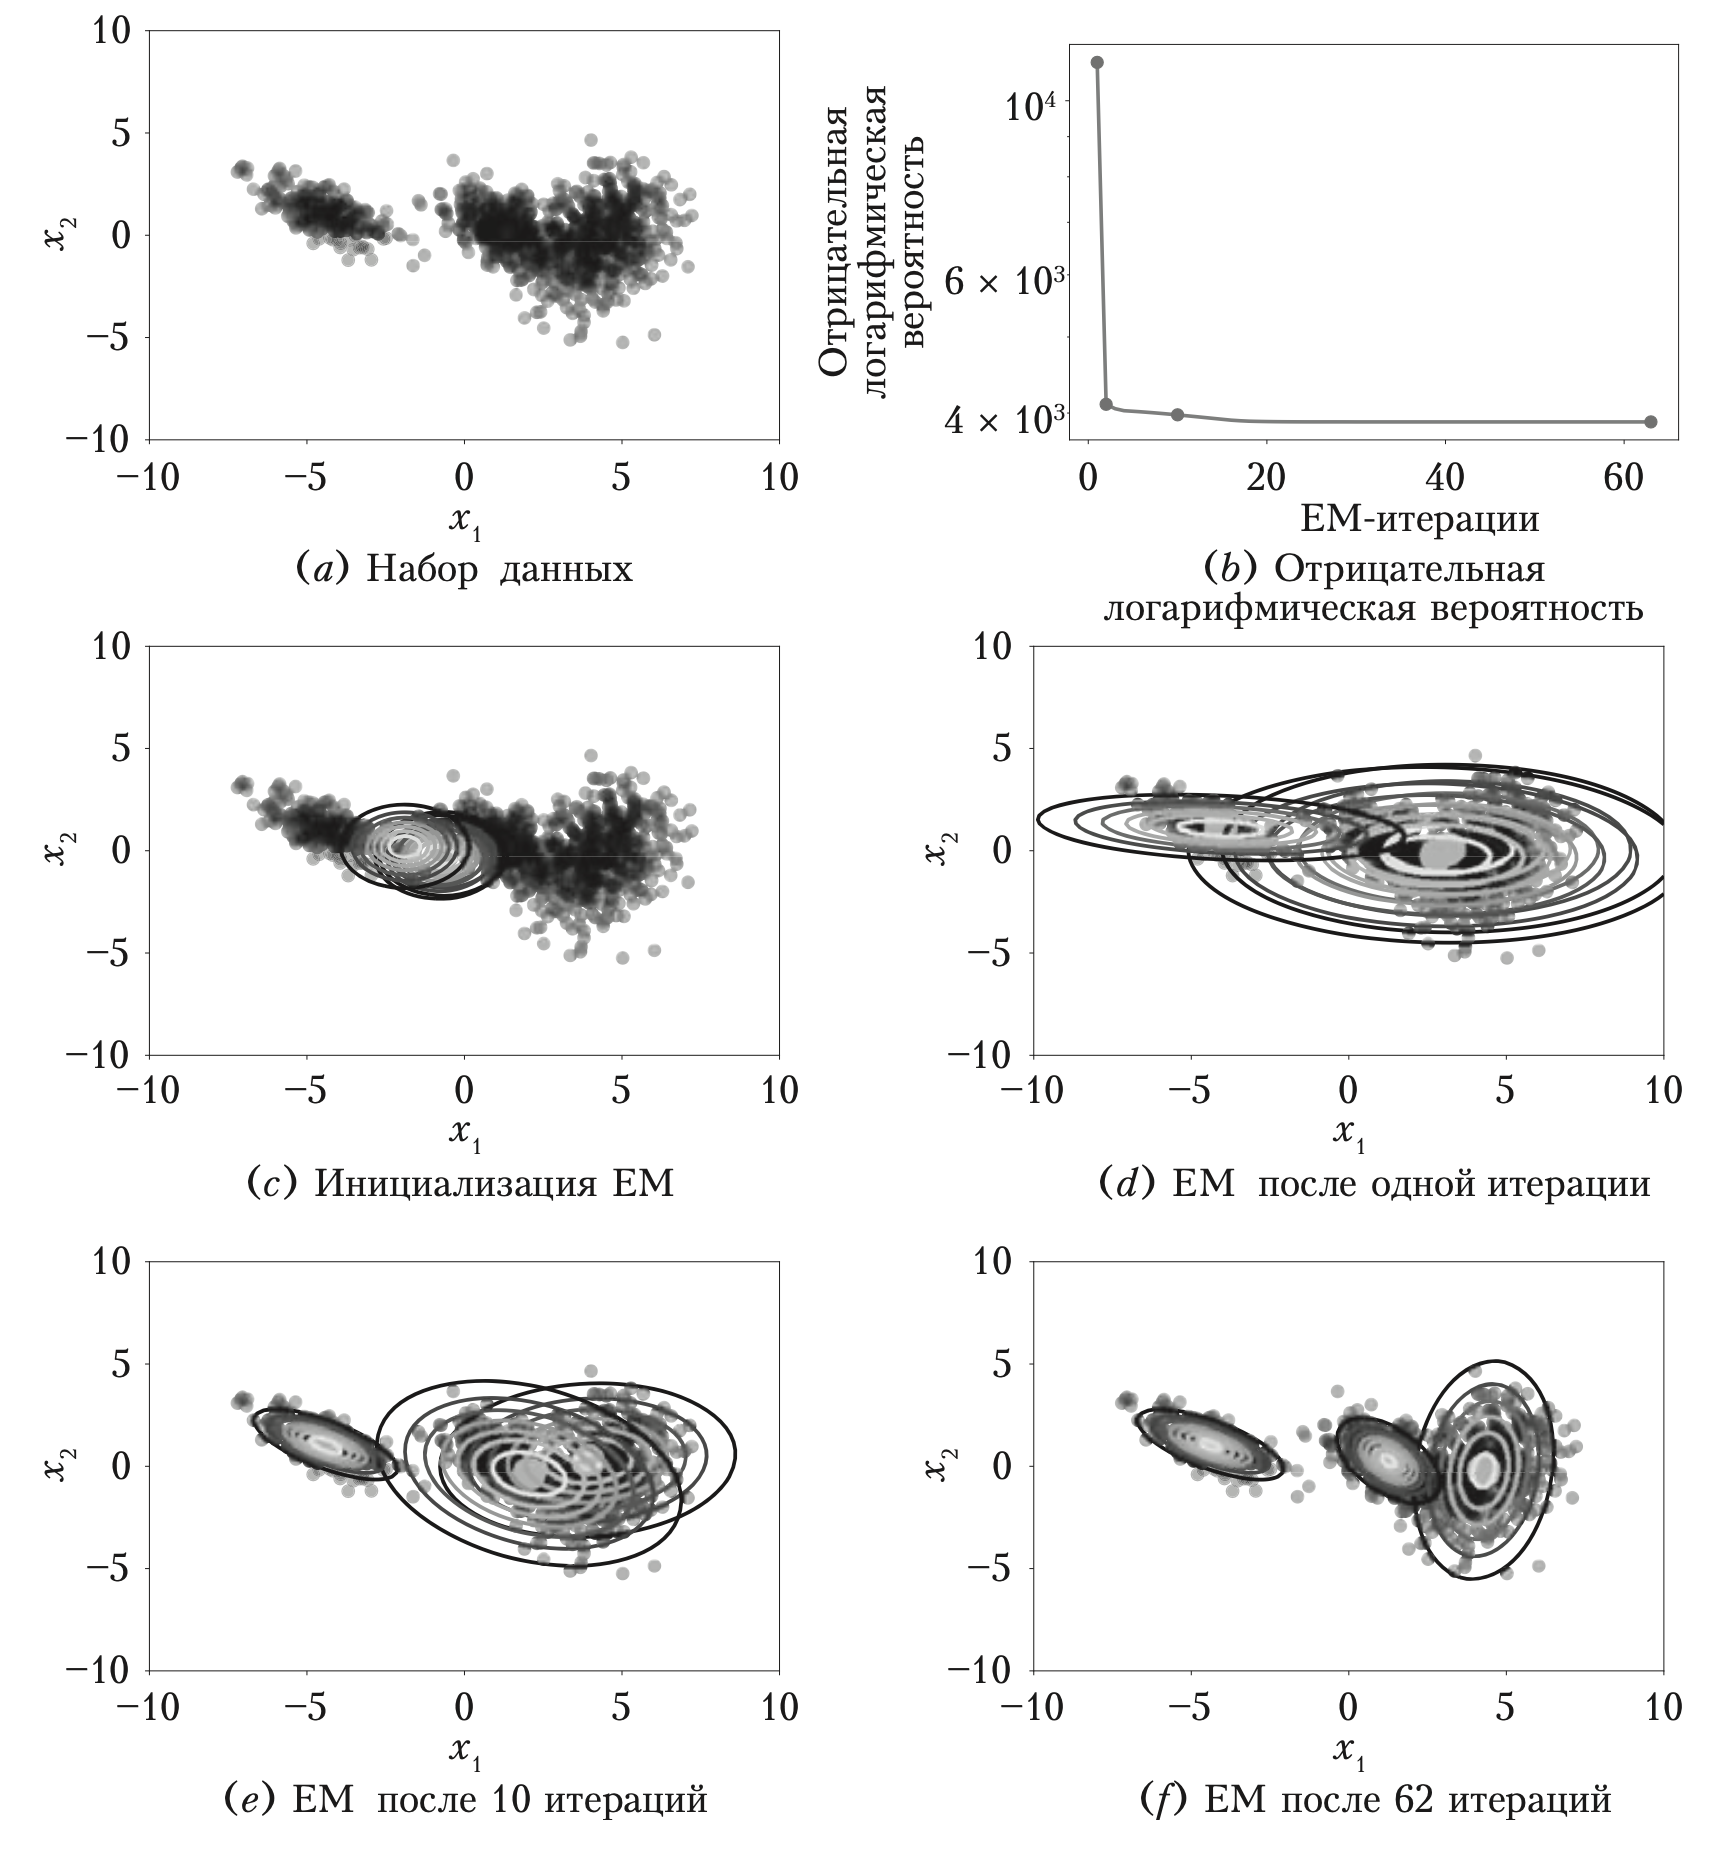
\includegraphics[width=\textwidth]{assets/em.png}
	\caption{Иллюстрация EM-алгоритма для обучения модели гауссовой смеси с тремя компонентами к двумерному набору данных}
	\label{fig:em}
\end{figure}



\section{Вывод}

В данном разделе был описан EM-алгоритм обучения модели гауссовой смеси. При фиксированном числе итераций алгоритма его временная трудоёмкость линейно зависит от числа точек в обучающем наборе данных и от числа компонент смеси.
